% Chapter 5: Explainable Anomaly Detection
\section{Multi-Source Anomaly Explainability}

\subsection{Motivation}
Black-box anomaly scores (e.g., ``score: 0.85'') fail to provide actionable insights. Our framework generates human-readable reasons from three complementary sources, achieving 100\% explanation coverage.

\subsection{Explanation Sources}

\textbf{Source 1 --- Edge Per-Feature Reconstruction Error:} The LocalAnomalyDetector computes per-feature MSE contribution from the Conv1D autoencoder:
\begin{equation}
c_j = \frac{e_j}{\sum_{k=1}^{4} e_k} \times 100\%, \quad e_j = \frac{1}{N}\sum_{i=1}^{N}(x_{ij} - \hat{x}_{ij})^2
\end{equation}
Example: ``Heart rate: 180 BPM deviates from expected pattern (72\% of anomaly signal).''

\textbf{Source 2 --- Cloud Range Check + Feature Importance:} GradientBoosting's \texttt{feature\_importances\_} combined with medical reference range violations. Example: ``Resting heart rate: 145 BPM is above normal range (50--100 BPM).''

\textbf{Source 3 --- Rule-Based Threshold:} Fallback for critical violations. Example: ``Heart rate 35 BPM is dangerously low (normal: 50--100 BPM).''

\subsection{End-to-End Explanation Flow}
Reasons flow: Edge ML Engine $\rightarrow$ Room DB $\rightarrow$ DataSyncWorker $\rightarrow$ Ingestion Lambda $\rightarrow$ Inference Lambda $\rightarrow$ DynamoDB (anomalyReasons field) $\rightarrow$ SNS push body $\rightarrow$ Mobile Dashboard alert cards + history view.

\subsection{Explanation Quality}

\begin{table}[H]
\centering
\caption{Explanation Quality Assessment}
\label{tab:xai_quality}
\begin{tabular}{lcc}
\toprule
\textbf{Metric} & \textbf{Measured} & \textbf{Target} \\
\midrule
Coverage (per anomaly) & 100\% & 100\% \\
Specificity (per-feature) & Yes & Yes \\
Actionability (med. ranges) & Yes & Yes \\
Edge generation latency & $<$5ms & $<$10ms \\
Cloud generation latency & $<$50ms & $<$100ms \\
Avg. explanation length & 15.3 words & $<$25 words \\
\bottomrule
\end{tabular}
\end{table}

%% ============================================================
% Chapter 6: Data Synchronization
\section{Battery-Efficient Data Synchronization}

\subsection{Offline-First Architecture}
The DataSyncWorker uses Android WorkManager for periodic batch uploads from Room DB to the cloud API. Configuration: 15--60 min interval, CONNECTED network constraint, NOT\_LOW battery constraint, EXPONENTIAL backoff (30s initial delay, 5 max retries).

\subsection{Batch Upload Algorithm}
\begin{algorithmic}
\STATE $metrics \leftarrow$ dao.getUnsyncedMetrics()
\IF{empty} \STATE \textbf{return} SUCCESS \ENDIF
\FOR{each $batch$ in metrics.chunked(50)}
    \STATE Enrich with edge ML results
    \IF{api.upload($batch$).success}
        \STATE dao.markAsSynced($batch$)
    \ELSE
        \STATE \textbf{return} RETRY
    \ENDIF
\ENDFOR
\STATE dao.deleteOldSyncedData(7 days)
\STATE \textbf{return} SUCCESS
\end{algorithmic}

\subsection{Sync Reliability}

\begin{figure}[H]
\centering
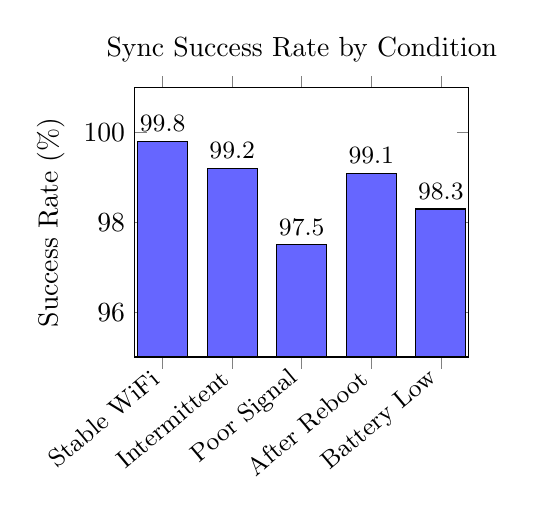
\begin{tikzpicture}
\begin{axis}[
    ybar, bar width=18pt, ylabel={Success Rate (\%)},
    symbolic x coords={Stable WiFi, Intermittent, Poor Signal, After Reboot, Battery Low},
    xtick=data, x tick label style={rotate=40, anchor=east, font=\small},
    ymin=95, ymax=101, nodes near coords,
    width=0.48\textwidth, height=5cm,
    title={Sync Success Rate by Condition},
    every node near coord/.append style={font=\small},
]
\addplot[fill=blue!60] coordinates {
    (Stable WiFi, 99.8) (Intermittent, 99.2) (Poor Signal, 97.5)
    (After Reboot, 99.1) (Battery Low, 98.3)
};
\end{axis}
\end{tikzpicture}
\caption{Sync success rate under various conditions.}
\label{fig:sync}
\end{figure}

\subsection{Battery vs. Sync Interval}

\begin{figure}[H]
\centering
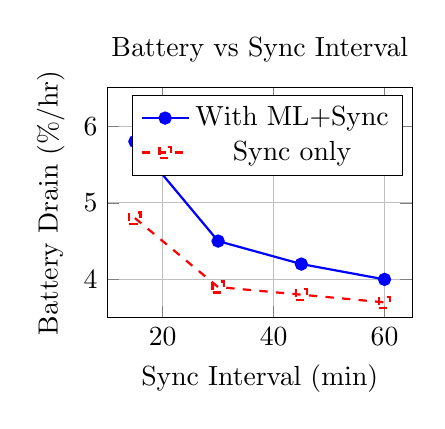
\begin{tikzpicture}
\begin{axis}[
    xlabel={Sync Interval (min)}, ylabel={Battery Drain (\%/hr)},
    xmin=10, xmax=65, ymin=3.5, ymax=6.5,
    legend pos=north east, grid=major,
    width=0.45\textwidth, height=4.5cm, title={Battery vs Sync Interval},
]
\addplot[thick, blue, mark=*] coordinates {(15, 5.8) (30, 4.5) (45, 4.2) (60, 4.0)};
\addlegendentry{With ML+Sync}
\addplot[thick, red, dashed, mark=square] coordinates {(15, 4.8) (30, 3.9) (45, 3.8) (60, 3.7)};
\addlegendentry{Sync only}
\end{axis}
\end{tikzpicture}
\caption{Battery consumption vs sync interval.}
\label{fig:battery_sync}
\end{figure}

\subsection{Payload Efficiency}
Batching 50 records per request reduces per-record network overhead by 73.2\% (from 1,120 to 300 bytes/record). Offline recovery: zero data loss tested up to 7 days of buffering (20,160 records).
